\documentclass[11pt]{article}
\usepackage[hmargin=1in,vmargin=1in]{geometry}
\usepackage[table]{xcolor} 
\usepackage{amsmath,amssymb,amsfonts,url,sectsty,tcolorbox,framed}
\usepackage{hyperref}
\usepackage{listings}
\usepackage{booktabs}
\usepackage{array}
\usepackage{multirow}
\usepackage{graphicx}
\usepackage{tikz}
\usetikzlibrary{arrows.meta, positioning, shapes.geometric, fit, backgrounds, calc}
\usepackage{pgfplots}
\pgfplotsset{compat=1.18}
\usepackage{fancyhdr}
\usepackage{fontawesome5}
\usepackage{enumitem}

% ──────────────────────────────────────────────────────
% COLOR PALETTE
% ──────────────────────────────────────────────────────
\definecolor{lightblue}{rgb}{0.8,0.9,1}
\definecolor{codebg}{RGB}{250, 250, 250}
\definecolor{codeframe}{RGB}{200, 200, 200}
\definecolor{tableheader}{RGB}{41, 128, 185}
\definecolor{rowalt}{RGB}{235, 245, 251}
\definecolor{accentblue}{RGB}{52, 152, 219}
\definecolor{accentgreen}{RGB}{39, 174, 96}
\definecolor{accentorange}{RGB}{230, 126, 34}
\definecolor{accentred}{RGB}{231, 76, 60}
\definecolor{accentpurple}{RGB}{142, 68, 173}
\definecolor{darkbg}{RGB}{30, 30, 30}
\definecolor{codekw}{RGB}{86, 156, 214}
\definecolor{codecomment}{RGB}{106, 153, 85}
\definecolor{codestring}{RGB}{206, 145, 120}
\definecolor{codenumber}{RGB}{181, 206, 168}
\definecolor{codetype}{RGB}{78, 201, 176}
\definecolor{sectioncolor}{RGB}{41, 128, 185}

% ──────────────────────────────────────────────────────
% SECTION STYLING
% ──────────────────────────────────────────────────────
\sectionfont{\color{sectioncolor}}
\subsectionfont{\color{sectioncolor!80!black}}
\subsubsectionfont{\color{sectioncolor!60!black}}

% ──────────────────────────────────────────────────────
% HYPERLINK STYLING
% ──────────────────────────────────────────────────────
\hypersetup{
    colorlinks=true,
    linkcolor=sectioncolor,
    urlcolor=accentblue,
    citecolor=accentgreen,
    pdfborder={0 0 0}
}

% ──────────────────────────────────────────────────────
% HEADER / FOOTER
% ──────────────────────────────────────────────────────
\pagestyle{fancy}
\fancyhf{}
\fancyhead[L]{\small\color{gray}\textsc{Lab 5: Parallel N-Queens}}
\fancyhead[R]{\small\color{gray}\textsc{CS302 -- DPC}}
\fancyfoot[C]{\small\color{gray}\thepage}
\renewcommand{\headrulewidth}{0.4pt}
\renewcommand{\footrulewidth}{0pt}
\fancypagestyle{plain}{\fancyhf{}\fancyfoot[C]{\small\color{gray}\thepage}\renewcommand{\headrulewidth}{0pt}}

% ──────────────────────────────────────────────────────
% CODE STYLE CONFIGURATION (VS Code Dark+ inspired)
% ──────────────────────────────────────────────────────
\lstset{
    backgroundcolor=\color{darkbg},
    basicstyle=\ttfamily\small\color{white},
    breaklines=true,
    breakatwhitespace=false,
    commentstyle=\color{codecomment}\itshape,
    keywordstyle=\color{codekw}\bfseries,
    stringstyle=\color{codestring},
    numberstyle=\tiny\color{gray},
    numbers=left,
    numbersep=8pt,
    stepnumber=1,
    frame=none,
    showstringspaces=false,
    language=C++,
    tabsize=4,
    columns=fullflexible,
    keepspaces=true,
    xleftmargin=10pt,
    morekeywords={omp_set_num_threads, omp_get_thread_num, omp_get_wtime, auto},
    emphstyle={\color{codetype}},
    emph={int, bool, long, double, void, const},
    literate=
        {0}{{\textcolor{codenumber}{0}}}1
        {1}{{\textcolor{codenumber}{1}}}1
        {2}{{\textcolor{codenumber}{2}}}1
        {3}{{\textcolor{codenumber}{3}}}1
        {4}{{\textcolor{codenumber}{4}}}1
        {5}{{\textcolor{codenumber}{5}}}1
        {6}{{\textcolor{codenumber}{6}}}1
        {7}{{\textcolor{codenumber}{7}}}1
        {8}{{\textcolor{codenumber}{8}}}1
        {9}{{\textcolor{codenumber}{9}}}1
        {\#pragma}{{\textcolor{accentpurple}{\#pragma}}}7
}

% ──────────────────────────────────────────────────────
% BOX DEFINITIONS
% ──────────────────────────────────────────────────────
\tcbuselibrary{breakable, skins, listings}

% Code block box (dark themed)
\newtcolorbox{codebox}[1][]{%
    enhanced,
    breakable,
    colback=darkbg,
    colframe=darkbg!60!black,
    title={\faCode\ \ #1},
    fonttitle=\bfseries\sffamily\small\color{white},
    coltitle=white,
    arc=4pt,
    boxrule=0.8pt,
    top=2pt,
    bottom=2pt,
    left=0pt,
    right=4pt,
    before skip=10pt,
    after skip=10pt,
    shadow={1mm}{-1mm}{0mm}{black!30},
    attach boxed title to top left={xshift=10pt, yshift=-\tcboxedtitleheight/2},
    boxed title style={colback=accentblue, arc=3pt, boxrule=0pt, left=6pt, right=6pt}
}

% Explanation / concept box
\newtcolorbox{shadedbox}[1][]{%
    enhanced,
    breakable,
    colback=lightblue!15,
    colframe=accentblue,
    title={\faLightbulb[regular]\ \ #1},
    fonttitle=\bfseries\sffamily,
    coltitle=white,
    arc=4pt,
    boxrule=0.8pt,
    before skip=10pt,
    after skip=10pt,
    shadow={1mm}{-1mm}{0mm}{accentblue!20},
    attach boxed title to top left={xshift=10pt, yshift=-\tcboxedtitleheight/2},
    boxed title style={colback=accentblue, arc=3pt, boxrule=0pt, left=6pt, right=6pt}
}

% Terminal output box
\newtcolorbox{terminalbox}[1]{%
    enhanced,
    breakable,
    colback=darkbg,
    colframe=darkbg!40!black,
    colupper=white,
    title={\faTerminal\ \ #1},
    fonttitle=\bfseries\ttfamily\small\color{white},
    coltitle=white,
    arc=4pt,
    boxrule=0.8pt,
    before skip=10pt,
    after skip=10pt,
    shadow={1mm}{-1mm}{0mm}{black!30},
    attach boxed title to top left={xshift=10pt, yshift=-\tcboxedtitleheight/2},
    boxed title style={colback=accentgreen!80!black, arc=3pt, boxrule=0pt, left=6pt, right=6pt}
}

% Warning / important box
\newtcolorbox{warningbox}[1][]{%
    enhanced,
    breakable,
    colback=accentorange!8,
    colframe=accentorange,
    title={\faExclamationTriangle\ \ #1},
    fonttitle=\bfseries\sffamily,
    coltitle=white,
    arc=4pt,
    boxrule=0.8pt,
    before skip=10pt,
    after skip=10pt,
    attach boxed title to top left={xshift=10pt, yshift=-\tcboxedtitleheight/2},
    boxed title style={colback=accentorange, arc=3pt, boxrule=0pt, left=6pt, right=6pt}
}

% Style for the code within the terminal
\lstdefinestyle{terminalstyle}{
    basicstyle=\ttfamily\small\color{white},
    breaklines=true,
    language=bash,
    numbers=none,
    literate={>}{{\textcolor{accentgreen}{>}}}1,
    columns=fullflexible,
    keepspaces=true,
    frame=none,
    backgroundcolor=\color{darkbg},
    xleftmargin=8pt
}

% Style for bash commands
\lstdefinestyle{bashstyle}{
    language=bash,
    basicstyle=\ttfamily\small\color{white},
    backgroundcolor=\color{darkbg},
    keywordstyle=\color{accentgreen}\bfseries,
    commentstyle=\color{gray}\itshape,
    numbers=none,
    frame=none,
    xleftmargin=8pt,
    breaklines=true,
    columns=fullflexible,
    keepspaces=true
}

\begin{document}

% ══════════════════════════════════════════════════════
% TITLE PAGE
% ══════════════════════════════════════════════════════
\thispagestyle{empty}
\begin{center}
\vspace*{1cm}

{\color{sectioncolor}\rule{\textwidth}{2pt}}
\vspace{0.3cm}

{\Huge\bfseries\sffamily\color{sectioncolor} Parallel N-Queens Solver}

\vspace{0.15cm}
{\Large\sffamily\color{gray} Backtracking with OpenMP Parallelization}

\vspace{0.3cm}
{\color{sectioncolor}\rule{\textwidth}{2pt}}

\vspace{1.2cm}

{\large\sffamily\color{sectioncolor} [CS302] Distributed and Parallel Computing}

\vspace{1.5cm}


\begin{tikzpicture}
\node[draw=sectioncolor, fill=sectioncolor!5, rounded corners=8pt, inner sep=15pt, minimum width=10cm] {
    \begin{tabular}{r @{\hspace{12pt}} l}
    \textbf{\color{sectioncolor}Course Instructor} & Dr. Sanjay Saxena \\
    \textbf{\color{sectioncolor}Session} & Winter 2026-27 \\
    \textbf{\color{sectioncolor}Submitted by} & Manveer Anand \\
    \textbf{\color{sectioncolor}Roll Number} & 202351080 \\
    \textbf{\color{sectioncolor}Assignment} & Lab 5 \\
    \end{tabular}
};
\end{tikzpicture}

\vspace{1.5cm}

{\color{gray}\small OpenMP Concepts: \texttt{parallel for} $\cdot$ \texttt{reduction} $\cdot$ \texttt{schedule(dynamic)} $\cdot$ \texttt{backtracking}}

\vfill
{\color{gray}\small\today}
\end{center}
\newpage

\tableofcontents
\newpage

% ══════════════════════════════════════════════════════
% INTRODUCTION
% ══════════════════════════════════════════════════════
\section{Introduction}

The N-Queens problem is a classical combinatorial problem in computer science: place $N$ queens on an $N \times N$ chessboard such that no two queens attack each other. Two queens attack each other if they share the same row, column, or diagonal.

For $N = 8$, the problem has \textbf{92} distinct solutions. This assignment implements a parallel solver using OpenMP that distributes the search space across multiple threads to count all valid configurations.

\subsection{Objectives}
\begin{enumerate}
    \item Place 8 queens on an $8 \times 8$ chessboard with no mutual attacks.
    \item Use OpenMP parallel programming to explore multiple placements concurrently.
    \item Calculate the total number of valid solutions.
    \item Measure and display execution time.
\end{enumerate}

\subsection{Attack Constraints}

A queen placed at position $(r_1, c_1)$ attacks another queen at $(r_2, c_2)$ if any of the following hold:

\begin{shadedbox}[Queen Attack Rules]
\begin{itemize}
    \item \textbf{Same row:} $r_1 = r_2$
    \item \textbf{Same column:} $c_1 = c_2$
    \item \textbf{Same diagonal:} $|r_1 - r_2| = |c_1 - c_2|$
\end{itemize}
Since we place exactly one queen per row (by construction), only the column and diagonal constraints need runtime checking.
\end{shadedbox}

\subsection{Example: N = 4}

For $N = 4$, there are exactly \textbf{2} valid solutions:

\begin{center}
\begin{tikzpicture}[scale=0.55]
    % Board 1
    \node[above] at (2, 4.3) {\sffamily\small\textbf{Solution 1}};
    \foreach \r/\c in {0/1, 1/3, 2/0, 3/2} {
        \fill[accentblue!20] (\c, 3-\r) rectangle (\c+1, 4-\r);
        \node at (\c+0.5, 3.5-\r) {\faChess};
    }
    \draw[step=1, gray, thin] (0,0) grid (4,4);
    \draw[thick] (0,0) rectangle (4,4);

    % Board 2
    \begin{scope}[xshift=6cm]
    \node[above] at (2, 4.3) {\sffamily\small\textbf{Solution 2}};
    \foreach \r/\c in {0/2, 1/0, 2/3, 3/1} {
        \fill[accentgreen!20] (\c, 3-\r) rectangle (\c+1, 4-\r);
        \node at (\c+0.5, 3.5-\r) {\faChess};
    }
    \draw[step=1, gray, thin] (0,0) grid (4,4);
    \draw[thick] (0,0) rectangle (4,4);
    \end{scope}
\end{tikzpicture}
\end{center}

% ══════════════════════════════════════════════════════
% APPROACH
% ══════════════════════════════════════════════════════
\section{Approach and Architecture}

\subsection{Algorithm: Backtracking}

The solver uses a \textbf{row-by-row backtracking} strategy:

\begin{enumerate}
    \item Represent the board as a 1D array \texttt{board[N]} where \texttt{board[i] = col} means a queen is in row $i$, column $col$.
    \item For each row, try every column $0$ to $N-1$.
    \item Check if the placement is safe (no column or diagonal conflict with previously placed queens).
    \item If safe, recurse to the next row. If row $= N$, a valid solution is found.
    \item Backtrack and try the next column.
\end{enumerate}

\subsection{Parallelization Strategy}

The key insight is that the first-row queen placement creates \textbf{independent sub-trees}. If the queen in row 0 is in column $c$, the entire sub-tree for that choice can be explored without any shared state with sub-trees rooted at other columns.

\begin{center}
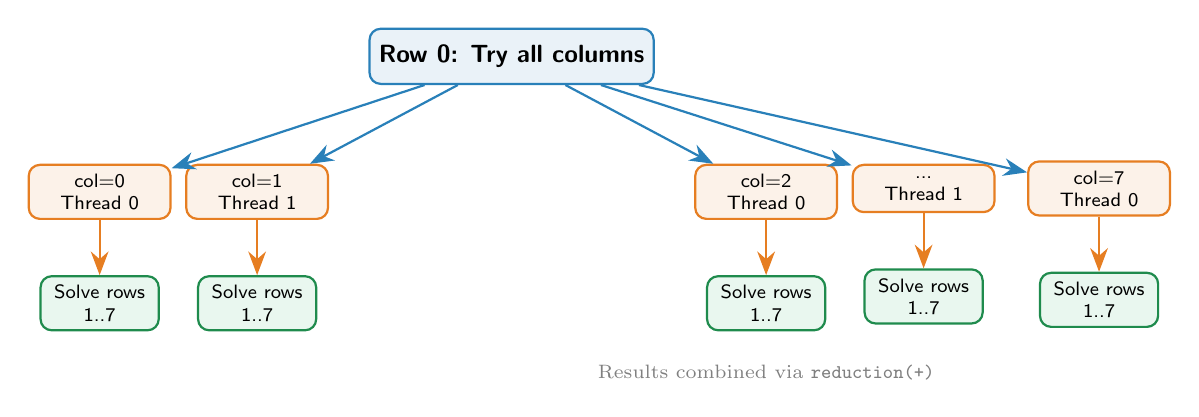
\begin{tikzpicture}[
    node distance=0.8cm and 0.6cm,
    >={Stealth[length=3mm]},
    rootbox/.style={rectangle, draw=sectioncolor, fill=sectioncolor!10, thick, rounded corners, minimum width=3cm, minimum height=0.7cm, font=\small\sffamily},
    threadbox/.style={rectangle, draw=accentorange, fill=accentorange!10, thick, rounded corners, minimum width=1.8cm, minimum height=0.6cm, font=\scriptsize\sffamily, align=center},
    leafbox/.style={rectangle, draw=accentgreen!80!black, fill=accentgreen!10, thick, rounded corners, minimum width=1.5cm, minimum height=0.5cm, font=\scriptsize\sffamily, align=center},
]
    \node[rootbox] (root) {\textbf{Row 0: Try all columns}};
    
    \node[threadbox, below left=1cm and 2.5cm of root] (t0) {col=0\\Thread 0};
    \node[threadbox, below left=1cm and 0.5cm of root] (t1) {col=1\\Thread 1};
    \node[threadbox, below right=1cm and 0.5cm of root] (t2) {col=2\\Thread 0};
    \node[threadbox, below right=1cm and 2.5cm of root] (t3) {...\\Thread 1};
    \node[threadbox, right=0.4cm of t3] (t7) {col=7\\Thread 0};

    \node[leafbox, below=0.7cm of t0] (s0) {Solve rows\\1..7};
    \node[leafbox, below=0.7cm of t1] (s1) {Solve rows\\1..7};
    \node[leafbox, below=0.7cm of t2] (s2) {Solve rows\\1..7};
    \node[leafbox, below=0.7cm of t3] (s3) {Solve rows\\1..7};
    \node[leafbox, below=0.7cm of t7] (s7) {Solve rows\\1..7};

    \draw[->, thick, sectioncolor] (root) -- (t0);
    \draw[->, thick, sectioncolor] (root) -- (t1);
    \draw[->, thick, sectioncolor] (root) -- (t2);
    \draw[->, thick, sectioncolor] (root) -- (t3);
    \draw[->, thick, sectioncolor] (root) -- (t7);

    \draw[->, thick, accentorange] (t0) -- (s0);
    \draw[->, thick, accentorange] (t1) -- (s1);
    \draw[->, thick, accentorange] (t2) -- (s2);
    \draw[->, thick, accentorange] (t3) -- (s3);
    \draw[->, thick, accentorange] (t7) -- (s7);

    \node[below=0.3cm of s2, font=\scriptsize\color{gray}] {Results combined via \texttt{reduction(+)}};
\end{tikzpicture}
\end{center}

\subsection{OpenMP Constructs Used}

\begin{center}
\sffamily\small
\begin{tabular}{@{}llp{7.5cm}@{}}
\toprule
\rowcolor{tableheader}
\textcolor{white}{\textbf{Construct}} & \textcolor{white}{\textbf{Directive}} & \textcolor{white}{\textbf{Purpose}} \\
\midrule
\rowcolor{rowalt}
Parallel For & \texttt{\#pragma omp parallel for} & Distributes first-row column choices across threads \\
Reduction & \texttt{reduction(+ : totalSolutions)} & Thread-safe accumulation of solution counts \\
\rowcolor{rowalt}
Dynamic Schedule & \texttt{schedule(dynamic)} & Balances load since sub-trees have unequal sizes \\
Wall Clock & \texttt{omp\_get\_wtime()} & High-resolution timing for execution measurement \\
\bottomrule
\end{tabular}
\end{center}

\begin{shadedbox}[Why \texttt{schedule(dynamic)}?]
Some first-row placements lead to larger search trees than others. For instance, placing a queen in a corner column prunes fewer branches than placing it near the center. Dynamic scheduling lets idle threads pick up the next unprocessed column, avoiding load imbalance.
\end{shadedbox}

\subsection{OpenMP Syntax Explained}

\subsubsection{\texttt{\#pragma omp parallel for}}

\begin{codebox}[Syntax: parallel for]
\begin{lstlisting}
#pragma omp parallel for schedule(dynamic) reduction(+ : totalSolutions)
for (int col = 0; col < N; col++)
{
    // body executed by multiple threads
}
\end{lstlisting}
\end{codebox}

This is a \textbf{combined directive} that does two things in one line:
\begin{itemize}
    \item \texttt{\#pragma omp parallel} --- creates a team of threads (fork).
    \item \texttt{for} --- distributes the loop iterations across those threads.
\end{itemize}
Without the \texttt{for} clause, every thread would execute the \textit{entire} loop. With it, OpenMP automatically splits iterations: e.g., with 4 threads and 8 iterations, each thread gets $\sim$2 iterations.

\subsubsection{\texttt{schedule(dynamic)}}

Controls \textit{how} iterations are assigned to threads:

\begin{center}
\sffamily\small
\begin{tabular}{@{}lp{9cm}@{}}
\toprule
\rowcolor{tableheader}
\textcolor{white}{\textbf{Schedule}} & \textcolor{white}{\textbf{Behavior}} \\
\midrule
\rowcolor{rowalt}
\texttt{static} & Iterations divided equally at compile time. Fast but assumes equal work per iteration. \\
\texttt{dynamic} & Each thread grabs the next unassigned iteration when it finishes. Handles unequal workloads. \\
\rowcolor{rowalt}
\texttt{guided} & Like dynamic but with decreasing chunk sizes. Good for gradually tapering workloads. \\
\bottomrule
\end{tabular}
\end{center}

We use \texttt{dynamic} because sub-trees rooted at different columns have different sizes.

\subsubsection{\texttt{reduction(+ : totalSolutions)}}

\begin{codebox}[Syntax: reduction]
\begin{lstlisting}
// Without reduction (WRONG -- race condition):
totalSolutions += localCount; // multiple threads write simultaneously

// With reduction (CORRECT):
#pragma omp parallel for reduction(+ : totalSolutions)
// Each thread gets a private copy of totalSolutions (initialized to 0).
// After the parallel region, all private copies are summed automatically.
\end{lstlisting}
\end{codebox}

The \texttt{reduction} clause tells OpenMP:
\begin{enumerate}
    \item Create a \textbf{private copy} of \texttt{totalSolutions} for each thread (initialized to the identity element: $0$ for \texttt{+}).
    \item Let each thread accumulate into its private copy freely (no synchronization).
    \item After all threads finish, \textbf{combine} all copies using the \texttt{+} operator.
\end{enumerate}
Other supported operators: \texttt{-}, \texttt{*}, \texttt{\&}, \texttt{|}, \texttt{\^{}}, \texttt{\&\&}, \texttt{||}, \texttt{min}, \texttt{max}.

\subsubsection{\texttt{omp\_get\_wtime()}}

\begin{codebox}[Syntax: Wall Clock Timing]
\begin{lstlisting}
double startTime = omp_get_wtime();  // returns seconds since an arbitrary point

// ... parallel computation ...

double endTime = omp_get_wtime();
double execTime = endTime - startTime;  // elapsed wall-clock seconds
\end{lstlisting}
\end{codebox}

\begin{itemize}
    \item Returns a \texttt{double} representing elapsed \textbf{wall-clock time} in seconds.
    \item Unlike \texttt{clock()} which measures CPU time (summed across cores), \texttt{omp\_get\_wtime()} measures real-world elapsed time --- the correct metric for parallel performance.
    \item The absolute value is meaningless; only the \textit{difference} between two calls matters.
\end{itemize}

\newpage

% ══════════════════════════════════════════════════════
% IMPLEMENTATION
% ══════════════════════════════════════════════════════
\section{Implementation}

\subsection{Safety Check}

\begin{codebox}[isSafe() -- Validate Queen Placement]
\begin{lstlisting}
bool isSafe(const int board[], int row, int col)
{
    for (int i = 0; i < row; i++)
    {
        // Same column or same diagonal
        if (board[i] == col || abs(board[i] - col) == abs(i - row))
            return false;
    }
    return true;
}
\end{lstlisting}
\end{codebox}

The function checks all previously placed queens (rows $0$ to $row-1$). Since we place one queen per row by construction, only column and diagonal conflicts need checking.

\subsection{Recursive Solver}

\begin{codebox}[solveNQueens() -- Backtracking Search]
\begin{lstlisting}
int solveNQueens(int board[], int row)
{
    if (row == N)
        return 1; // All queens placed successfully

    int count = 0;
    for (int col = 0; col < N; col++)
    {
        if (isSafe(board, row, col))
        {
            board[row] = col;
            count += solveNQueens(board, row + 1);
        }
    }
    return count;
}
\end{lstlisting}
\end{codebox}

This is a pure recursive function with no shared state---each call only reads/writes its own \texttt{board[]} array from \texttt{row} onwards. This property makes it safe for parallel execution.

\subsection{Parallel Driver}

\begin{codebox}[main() -- OpenMP Parallel Search]
\begin{lstlisting}
int totalSolutions = 0;

double startTime = omp_get_wtime();

// Parallelize over first-row queen placements
#pragma omp parallel for schedule(dynamic) reduction(+ : totalSolutions)
for (int col = 0; col < N; col++)
{
    int localBoard[N];
    localBoard[0] = col;
    totalSolutions += solveNQueens(localBoard, 1);
}

double endTime = omp_get_wtime();
double execTime = endTime - startTime;
\end{lstlisting}
\end{codebox}

\begin{shadedbox}[Key Design Decisions]
\textbf{1. Each thread gets its own \texttt{localBoard[]} array.} \\
Declared inside the parallel for loop, so it's private to each thread. No synchronization needed for board access.

\vspace{6pt}
\textbf{2. \texttt{reduction(+: totalSolutions)}} \\
Each thread accumulates its sub-tree count in a private copy. After all iterations complete, OpenMP automatically sums them into the shared \texttt{totalSolutions}. This avoids any critical sections or atomic operations.

\vspace{6pt}
\textbf{3. Parallelism at row 0 only} \\
With $N = 8$ columns at row 0, there are 8 independent tasks---enough to keep threads busy without the overhead of task-level parallelism deeper in the tree.
\end{shadedbox}

\subsection{Sample Solution Printer}

\begin{codebox}[findFirst() -- Lambda for First Valid Board]
\begin{lstlisting}
auto findFirst = [&](int board[], int row, auto &self) -> bool
{
    if (row == N)
        return true;
    for (int col = 0; col < N; col++)
    {
        if (isSafe(board, row, col))
        {
            board[row] = col;
            if (self(board, row + 1, self))
                return true;
        }
    }
    return false;
};
\end{lstlisting}
\end{codebox}

This recursive lambda finds the \textit{first} valid configuration and stops (unlike \texttt{solveNQueens} which counts all). It uses the C++14 generic lambda self-reference pattern.

\newpage

% ══════════════════════════════════════════════════════
% OUTPUT
% ══════════════════════════════════════════════════════
\section{Program Output}

\begin{terminalbox}{N = 8 -- Parallel 8-Queens Solver}
\begin{lstlisting}[style=terminalstyle]
========================================
  Parallel 8-Queens Solver (OpenMP)
========================================
Board Size: 8 x 8

Total Valid Solutions : 92
Execution Time       : 0.00200009 seconds

-- Sample Valid Configuration --
 Q . . . . . . .
 . . . . Q . . .
 . . . . . . . Q
 . . . . . Q . .
 . . Q . . . . .
 . . . . . . Q .
 . Q . . . . . .
 . . . Q . . . .
========================================
\end{lstlisting}
\end{terminalbox}

The program correctly finds all \textbf{92} solutions for the 8-Queens problem, which matches the known mathematical result.

% ══════════════════════════════════════════════════════
% KNOWN SOLUTIONS TABLE
% ══════════════════════════════════════════════════════
\section{N-Queens: Known Solution Counts}

\begin{table}[htbp]
\centering
\sffamily\small
\caption{Number of Solutions for Various Board Sizes}
\vspace{6pt}
\begin{tabular}{@{}cc@{}}
\toprule
\rowcolor{tableheader}
\textcolor{white}{\textbf{N}} & \textcolor{white}{\textbf{Total Solutions}} \\
\midrule
\rowcolor{rowalt}
1 & 1 \\
2 & 0 \\
\rowcolor{rowalt}
3 & 0 \\
4 & 2 \\
\rowcolor{rowalt}
5 & 10 \\
6 & 4 \\
\rowcolor{rowalt}
7 & 40 \\
\textbf{8} & \textbf{92} \\
\rowcolor{rowalt}
9 & 352 \\
10 & 724 \\
\rowcolor{rowalt}
12 & 14,200 \\
13 & 73,712 \\
\bottomrule
\end{tabular}
\end{table}

Our program's output of \textbf{92} for $N = 8$ is verified correct against the known sequence.

\newpage

% ══════════════════════════════════════════════════════
% COMPLEXITY ANALYSIS
% ══════════════════════════════════════════════════════
\section{Complexity Analysis}

\subsection{Time Complexity}

\begin{shadedbox}[Sequential Complexity]
\textbf{Worst case:} The algorithm explores all possible column placements across all rows: $N$ choices per row, $N$ rows deep.

$$T_{\text{worst}} = O(N^N)$$

\textbf{With pruning:} Backtracking prunes invalid branches early. The effective number of nodes explored is much smaller, but no closed-form exists. For $N = 8$, only $\sim$15,720 nodes are visited (vs. $8^8 = 16,777,216$ without pruning).

\vspace{4pt}
\textbf{isSafe() per call:} $O(N)$ --- checks all previously placed queens.

\vspace{4pt}
\textbf{Effective complexity:} $O(N! \cdot N)$ is a reasonable practical bound, since each row has progressively fewer valid columns.
\end{shadedbox}

\subsection{Space Complexity}

\begin{shadedbox}[Memory Usage]
\textbf{Board representation:} $O(N)$ --- one integer per row.

\vspace{4pt}
\textbf{Recursion stack:} $O(N)$ --- maximum depth is $N$ rows.

\vspace{4pt}
\textbf{Parallel overhead:} $O(N \cdot T)$ --- each of $T$ threads maintains its own board array.

\vspace{4pt}
\textbf{Total:} $O(N \cdot T)$ where $T$ is the thread count.
\end{shadedbox}

\subsection{Parallelism Analysis}

With $N = 8$ first-row columns distributed across threads:

\begin{itemize}
    \item \textbf{Maximum parallelism:} $N = 8$ independent tasks.
    \item \textbf{Granularity:} Each task is a full sub-tree search (rows 1--7), providing sufficient work per thread.
    \item \textbf{Load balance:} Sub-trees are unequal in size. Column 0 and column 7 (corners) generate fewer valid placements than central columns. \texttt{schedule(dynamic)} compensates for this imbalance.
    \item \textbf{Synchronization:} Zero during computation---\texttt{reduction} handles the final sum.
\end{itemize}

% ══════════════════════════════════════════════════════
% TECHNICAL DEEP DIVE
% ══════════════════════════════════════════════════════
\section{Technical Deep Dive}

\subsection{Why \texttt{reduction} Instead of \texttt{atomic} or \texttt{critical}?}

\begin{shadedbox}[Reduction vs. Alternatives]
\textbf{\texttt{\#pragma omp atomic}} --- Would work for a single \texttt{+=} but would be called once per sub-tree completion (8 times). At this granularity, either works fine.

\vspace{4pt}
\textbf{\texttt{\#pragma omp critical}} --- Overkill. Critical sections serialize thread execution and are meant for multi-statement blocks.

\vspace{4pt}
\textbf{\texttt{reduction(+: ...)}} --- The cleanest and most idiomatic approach. Each thread gets a private copy initialized to 0. The runtime combines them automatically after the parallel region. No explicit synchronization in user code.
\end{shadedbox}

\subsection{Board Representation: 1D Array vs. 2D Grid}

Using \texttt{board[row] = col} instead of an $N \times N$ boolean grid has key advantages:

\begin{itemize}
    \item \textbf{Memory:} $N$ integers vs. $N^2$ booleans.
    \item \textbf{Row uniqueness:} Guaranteed by construction---each index stores exactly one column.
    \item \textbf{Diagonal check:} Reduces to \texttt{abs(board[i] - col) == abs(i - row)}, which is $O(1)$ per pair.
    \item \textbf{Copy cost:} Only $N$ integers need copying for thread-local boards.
\end{itemize}

\subsection{Backtracking Pruning Effectiveness}

\begin{table}[htbp]
\centering
\sffamily\small
\caption{Search Space Pruning ($N = 8$)}
\vspace{6pt}
\begin{tabular}{@{}lr@{}}
\toprule
\rowcolor{tableheader}
\textcolor{white}{\textbf{Metric}} & \textcolor{white}{\textbf{Value}} \\
\midrule
\rowcolor{rowalt}
Total permutations ($N^N$) & 16,777,216 \\
Nodes actually explored & $\sim$15,720 \\
\rowcolor{rowalt}
Pruning ratio & 99.91\% \\
Valid solutions found & 92 \\
\bottomrule
\end{tabular}
\end{table}

Backtracking eliminates 99.91\% of the search space by detecting conflicts as early as possible.

% ══════════════════════════════════════════════════════
% COMPILATION
% ══════════════════════════════════════════════════════
\section{Compilation and Execution}

\subsection{Build Instructions}

\begin{codebox}[Build \& Run Commands]
\begin{lstlisting}[style=bashstyle]
# Compile with OpenMP support and optimization
g++ -fopenmp -O2 -o n_queens.exe n_queens.cpp

# Run the program
./n_queens.exe
\end{lstlisting}
\end{codebox}

\subsection{Compiler Flags}

\begin{center}
\sffamily\small
\begin{tabular}{@{}lp{10cm}@{}}
\toprule
\rowcolor{tableheader}
\textcolor{white}{\textbf{Flag}} & \textcolor{white}{\textbf{Purpose}} \\
\midrule
\rowcolor{rowalt}
\texttt{-fopenmp} & Enables OpenMP: recognizes \texttt{\#pragma omp} directives and links the runtime \\
\texttt{-O2} & Level 2 optimization: improves loop and recursion performance \\
\bottomrule
\end{tabular}
\end{center}

% ══════════════════════════════════════════════════════
% CONCLUSION
% ══════════════════════════════════════════════════════
\section{Conclusion}

This assignment demonstrates parallel backtracking search using OpenMP through the N-Queens problem. The solver correctly finds all \textbf{92} valid configurations for an $8 \times 8$ board. The parallelization strategy---distributing first-row column choices across threads with \texttt{reduction} for combining counts---is both simple and effective. The approach requires \textbf{zero synchronization} during the search phase, making it an ideal case study for embarrassingly parallel recursive computation. The same pattern generalizes to larger $N$ values, where the increased search space makes parallel speedup increasingly valuable.

\end{document}
